\chapter{Validação}\label{cap:validacao}

\section{Introdução}

Este capítulo apresenta separadamente os resultados tabulares e espaciais. O primeiro eixo usa a base legada de 40 execuções e 1.234 intervalos. O segundo usa subconjuntos documentados dos 103 diretórios de execuções espaciais completas. Essa separação é importante porque as execuções espaciais foram produzidas durante diferentes fases de desenvolvimento e não substituem a coorte tabular.

\section{Material e métodos}

\subsection{Divisão dos dados e métricas}

No eixo tabular, 35 execuções formam o treino final, duas compõem a validação fixa e três o teste fixo. Os marcos 9, 17, 25, 33 e 40 indicam o total de execuções disponível, mantendo sempre as mesmas cinco execuções reservadas. MAE, RMSE e correlação foram calculados nas unidades originais. Para eventos de proximidade também foram usados acurácia balanceada, precisão, revocação e F1.

No eixo espacial, a bateria final de referência contém as dez execuções consecutivas registradas entre \texttt{run\_20260831\_082418\_723471} e \texttt{run\_20260831\_084356\_708163}. O arquivo completo possui 103 diretórios de execuções completas, mas eles não formam um único conjunto: versões diferentes reutilizaram subconjuntos para desenvolvimento, treino e diagnóstico. Para evitar dupla contagem, cada diretório recebeu uma categoria principal exclusiva: 69 são de desenvolvimento e diagnóstico, 20 de treino da v19, dez da bateria final de referência, dois históricos reservados, um de calibração da v19 e um de desenvolvimento de modelos anteriores. Essas seis classes somam exatamente 103; execuções de foco e portão permanecem marcadores secundários porque se sobrepõem a essas classes.

\begin{table}[htb]
\centering
\caption{Classificação principal exclusiva das execuções espaciais.}
\label{tab:mono-composicao-espacial}
\begin{tabular}{lr}
\hline
Desenvolvimento e diagnóstico & 69 \\
Treino da v19 & 20 \\
Bateria final com profundidade do Gazebo & 10 \\
Conjuntos históricos reservados & 2 \\
Calibração da v19 & 1 \\
Desenvolvimento de modelos anteriores & 1 \\
Total & 103 \\
\hline
\end{tabular}
\legend{Fonte: inventário individual gerado pelo script de auditoria. Marcadores secundários podem se sobrepor às classes.}
\end{table}

\subsection{Composição da validação monocular}

A versão v19 usou 20 execuções completas no treino e uma execução separada apenas para calibração. As quatro execuções de foco são um subconjunto dessas 20 execuções, repetido de forma dirigida no treinamento. O treino efetivo registrou 3.322 quadros. A terceira execução da bateria final, \texttt{run\_20260831\_082836\_332335}, foi usada na validação durante o treinamento e também como conjunto primário do portão. Portanto, ela não é um teste independente.

Quatro conjuntos foram reservados para o estágio secundário: a sexta execução da bateria final, \texttt{run\_20260831\_083521\_770086}; a décima, \texttt{run\_20260831\_084356\_708163}; uma execução antiga independente, \texttt{run\_20260820\_225114\_611267}; e uma execução histórica reservada, \texttt{run\_20260819\_191346\_877996}. Nenhum participou do ajuste dos pesos da v19. Depois do congelamento do modelo e da configuração, os quatro foram executados offline.

O portão por pixel exigia simultaneamente MAE global de no máximo 2,0~m, AbsRel de no máximo 0,30, MAE até 5~m de no máximo 1,0~m, viés positivo até 5~m de no máximo 0,5~m, percentil 95 do erro positivo até 5~m de no máximo 1,25~m, MAE entre 5 e 10~m de no máximo 1,5~m e latência no percentil 95 de no máximo 400~ms. O portão espacial exigia: pelo menos 100 quadros integrados; caminho executável mínimo de 1,5~m; taxa de sucesso de planejamento igual ou superior a 80\%; taxa de falso espaço livre igual ou inferior a 10\%; ao menos um plano executável; e todos os planos executáveis livres de colisão no mapa produzido com profundidade do Gazebo.

\section{Evidências experimentais}

\subsection{Crescimento do conjunto e perdas}

A Figura~\ref{fig:mono-curva-aprendizado} mostra o MAE no teste fixo. Entre 9 e 40 execuções, o erro caiu em cinco dos seis alvos, mas os valores oscilaram nos marcos intermediários. A diversidade das novas execuções, e não apenas sua quantidade, afetou o resultado.

\begin{figure}[htb]
    \centering
    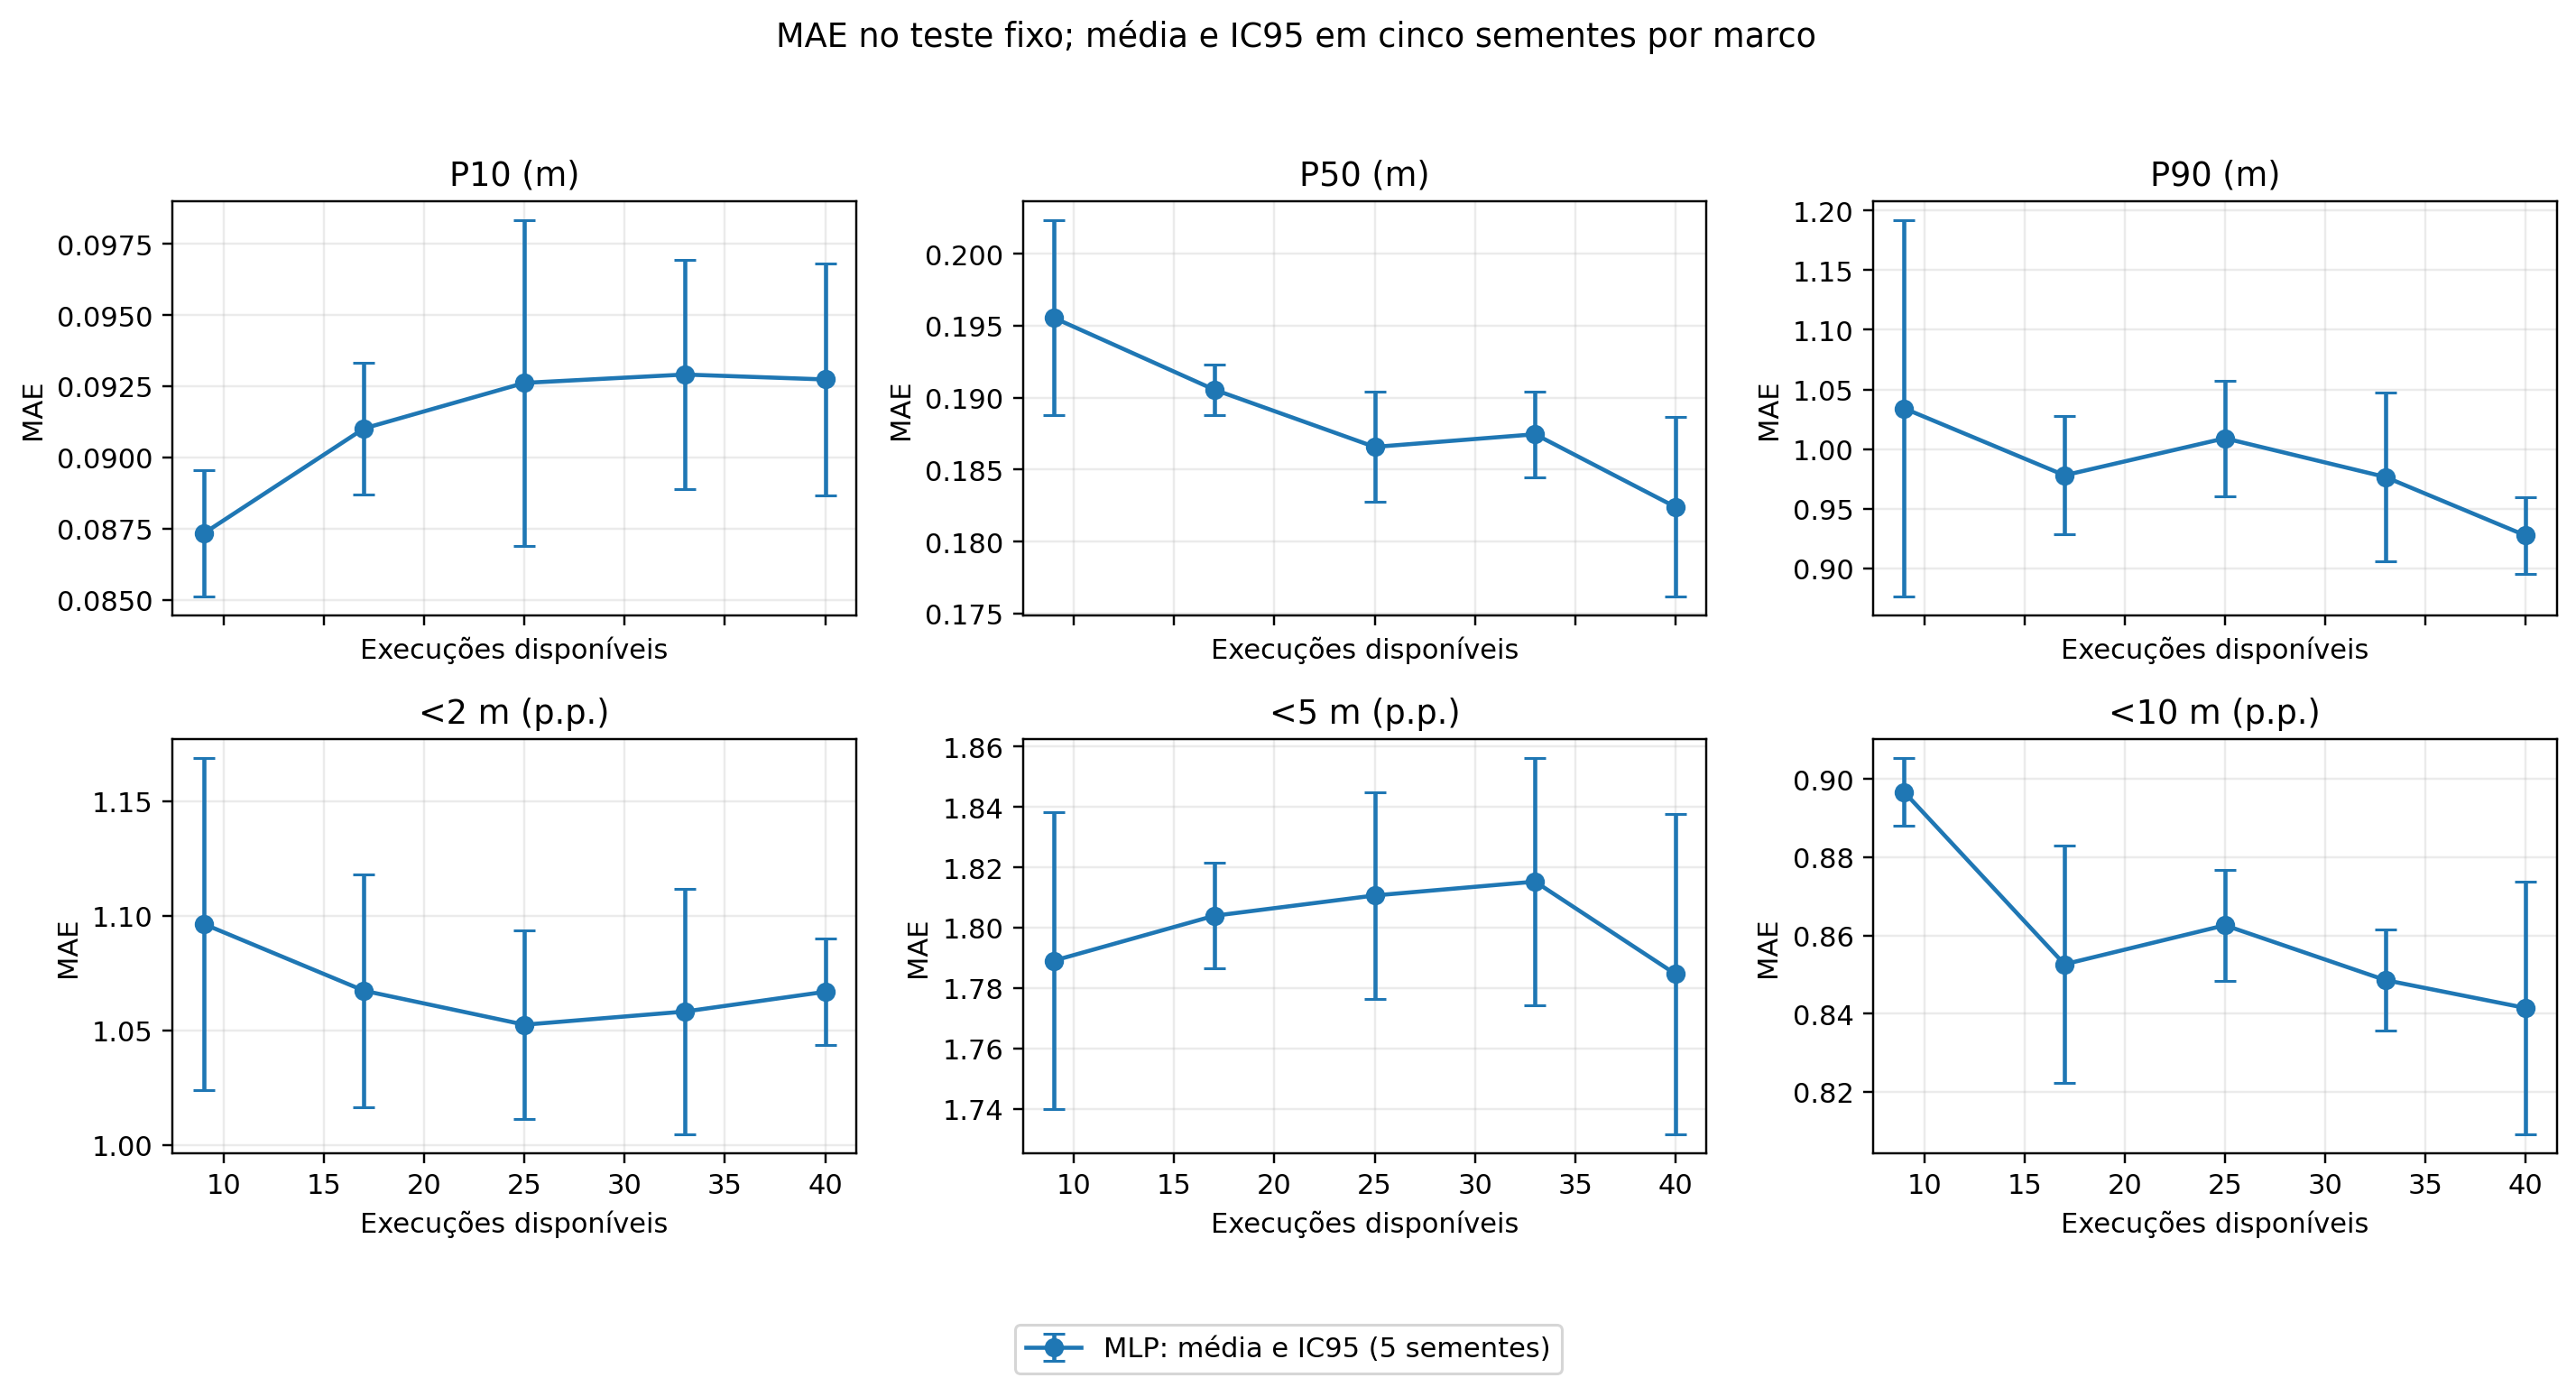
\includegraphics[width=\textwidth]{figuras/resultados_curva_aprendizado.png}
    \caption{MAE da MLP nos cinco marcos. As barras são IC95 da média entre cinco sementes, calculados com distribuição $t$ e $n=5$; representam variação algorítmica no mesmo teste fixo, não novas coletas.}
    \label{fig:mono-curva-aprendizado}
    \legend{Fonte: elaborado pelo autor.}
\end{figure}

A menor perda de validação ocorreu na época 17. O treinamento parou na época 67 e restaurou os pesos da época 17. A parada antecipada e a seleção dos pesos consideraram somente a perda de validação. A perda do teste foi calculada posteriormente para a figura e não participou do treinamento, da escolha da época ou do ajuste de hiperparâmetros. A Figura~\ref{fig:mono-loss} mostra que a perda de treino continuou caindo enquanto validação e teste deixaram de acompanhar essa melhora.

\begin{figure}[htb]
    \centering
    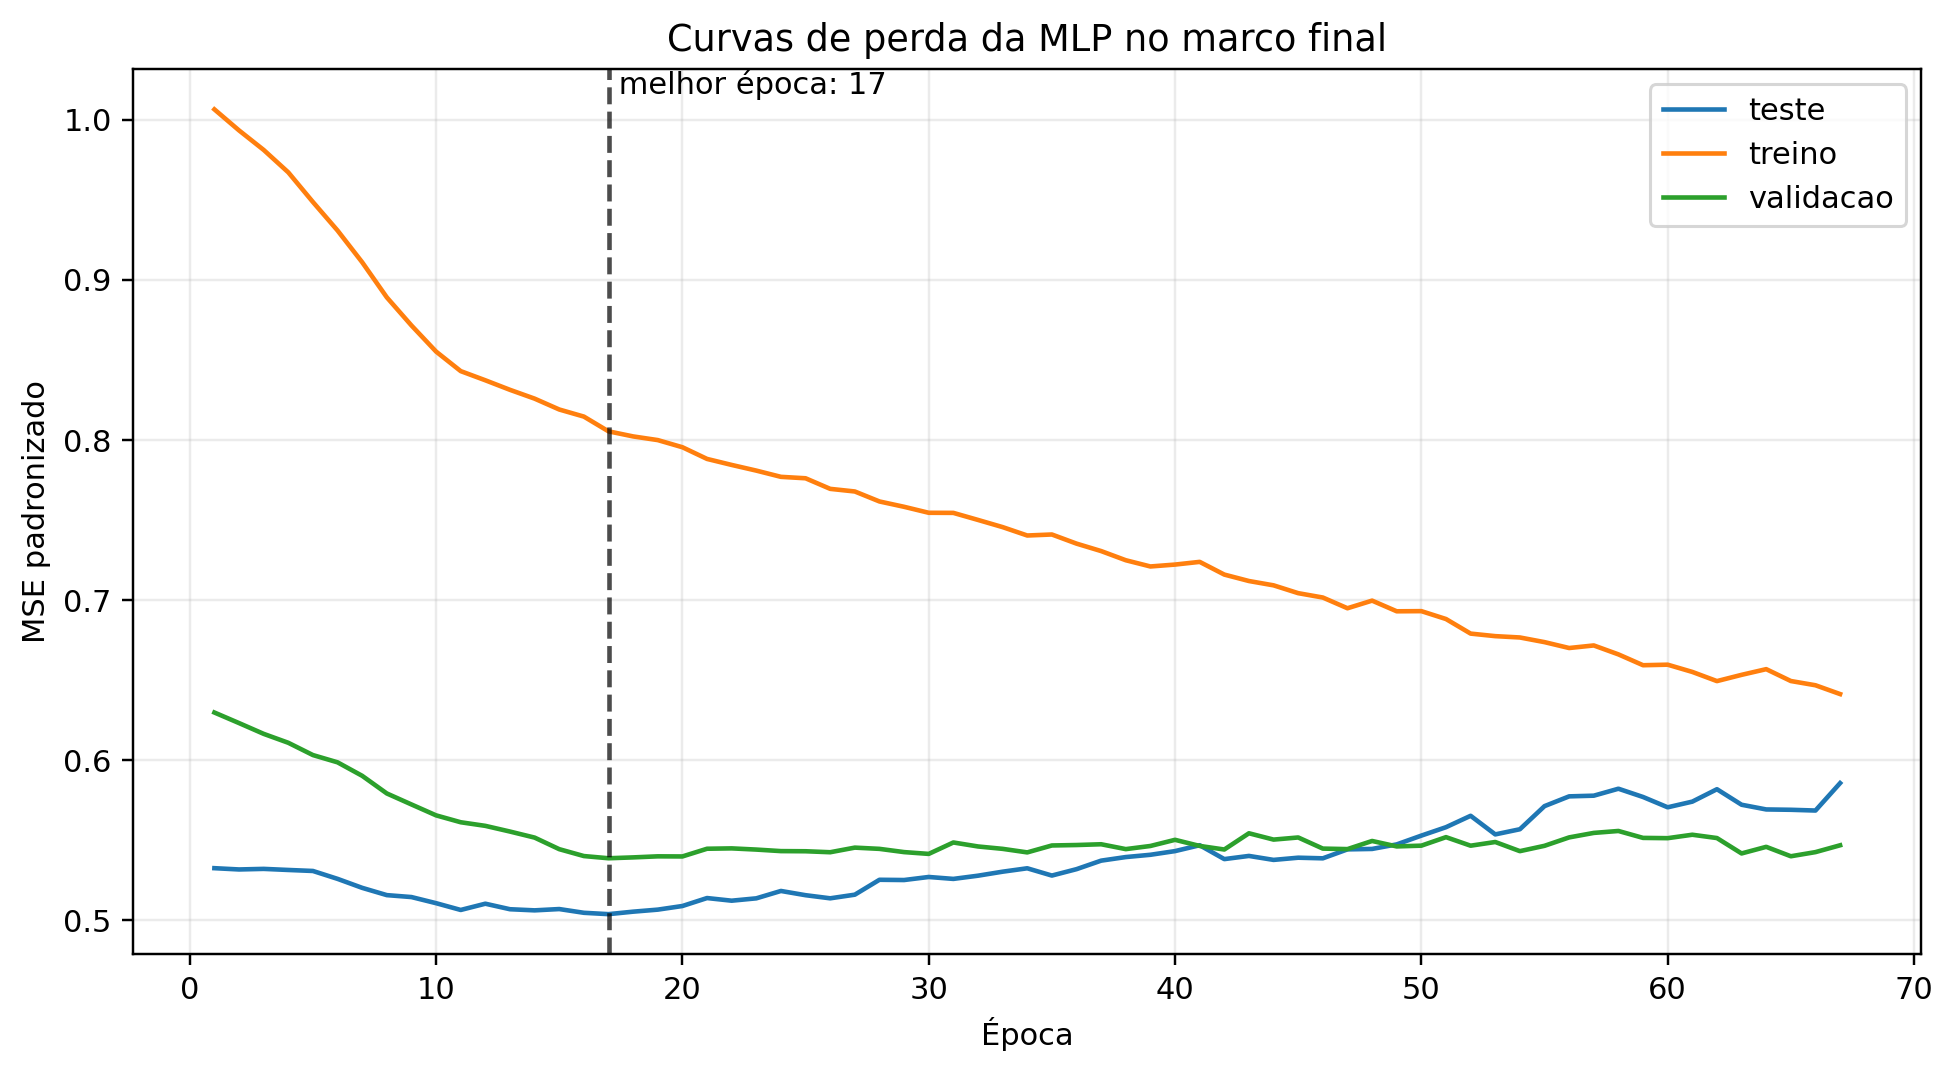
\includegraphics[width=\textwidth]{figuras/resultados_curvas_loss.png}
    \caption{Curvas de perda da MLP no marco final da base tabular.}
    \label{fig:mono-loss}
    \legend{Fonte: elaborado pelo autor.}
\end{figure}

\subsection{MLP, referências e estabilidade}

A Tabela~\ref{tab:mono-modelos} reúne o MAE do teste. MLP, Random Forest e Extra Trees são apresentadas pela média e pelo desvio padrão das mesmas cinco sementes, usando os mesmos conjuntos fixos. Nenhum modelo venceu em todos os alvos; para P10 e P90, a média do treino foi a melhor referência.

\begin{table}[htb]
\centering
\caption{MAE no teste fixo e estabilidade da MLP.}
\label{tab:mono-modelos}
\resizebox{\textwidth}{!}{%
\begin{tabular}{lcccc}
\hline
\textbf{Alvo} & \textbf{MLP média $\pm$ desvio} & \textbf{RF média $\pm$ desvio} & \textbf{ET média $\pm$ desvio} & \textbf{Média do treino} \\
\hline
$\Delta P10$ (m) & $0,0921 \pm 0,0034$ & $0,0884 \pm 0,0006$ & $0,0906 \pm 0,0004$ & \textbf{0,0867} \\
$\Delta P50$ (m) & $0,1820 \pm 0,0056$ & \textbf{$0,1766 \pm 0,0010$} & $0,1818 \pm 0,0019$ & 0,1886 \\
$\Delta P90$ (m) & $0,9259 \pm 0,0273$ & $0,9255 \pm 0,0031$ & $0,9421 \pm 0,0125$ & \textbf{0,8246} \\
$\Delta$ pixels $<2$ m (p.p.) & \textbf{$1,0566 \pm 0,0268$} & $1,0752 \pm 0,0033$ & $1,1250 \pm 0,0013$ & 1,0869 \\
$\Delta$ pixels $<5$ m (p.p.) & $1,7834 \pm 0,0436$ & \textbf{$1,7652 \pm 0,0116$} & $1,7978 \pm 0,0058$ & 1,8488 \\
$\Delta$ pixels $<10$ m (p.p.) & \textbf{$0,8423 \pm 0,0318$} & $0,8612 \pm 0,0043$ & $0,8773 \pm 0,0123$ & 0,9096 \\
\hline
\end{tabular}}
\legend{Fonte: elaborado pelo autor.}
\end{table}

O coeficiente de variação do MAE da MLP ficou entre 2,4\% e 3,8\%. A época escolhida variou de 22 a 182, mas o nível final de erro mudou pouco. No diagnóstico pareado, MLP--Random Forest apresentou $(d_z,p)$ de $(1,32;0,042)$, $(1,15;0,061)$ e $(0,08;0,868)$ para P10, P50 e P90, e $(-0,48;0,339)$, $(0,40;0,425)$ e $(-0,66;0,215)$ para os limiares de 2, 5 e 10~m. MLP--Extra Trees apresentou, na mesma ordem, $(0,72;0,184)$, $(0,11;0,824)$, $(-0,94;0,103)$, $(-3,13;0,002)$, $(-0,30;0,545)$ e $(-1,01;0,087)$. Com cinco pares e múltiplos alvos, esses resultados são exploratórios e não demonstram superioridade geral.

\subsection{Eventos, gradientes e ablação}

O classificador final de eventos obteve acurácia balanceada de 0,615, precisão de 0,789, revocação de 0,870 e F1 de 0,828. O pipeline completo teve MAE de 1,770 ponto percentual para pixels abaixo de 5~m. Quando a indicação real de evento foi fornecida somente para diagnóstico, o MAE caiu para 1,744. A diferença pequena indica que a regressão do sinal e da magnitude concentra a maior parte do erro.

A Figura~\ref{fig:mono-ablacao} compara gradientes e ablação. IMU e atitude reuniram 43,4\% da sensibilidade média e sua retirada elevou o MAE em 5,45\% na média agregada dos seis alvos. O efeito não foi uniforme: foi negativo em P90 e alguns IC95 por alvo incluíram zero. A Tabela~\ref{tab:mono-ablacao} mostra o efeito médio de cada grupo. Valores negativos significam que a retirada reduziu o erro médio, dentro da variabilidade observada entre sementes.

\begin{figure}[htb]
    \centering
    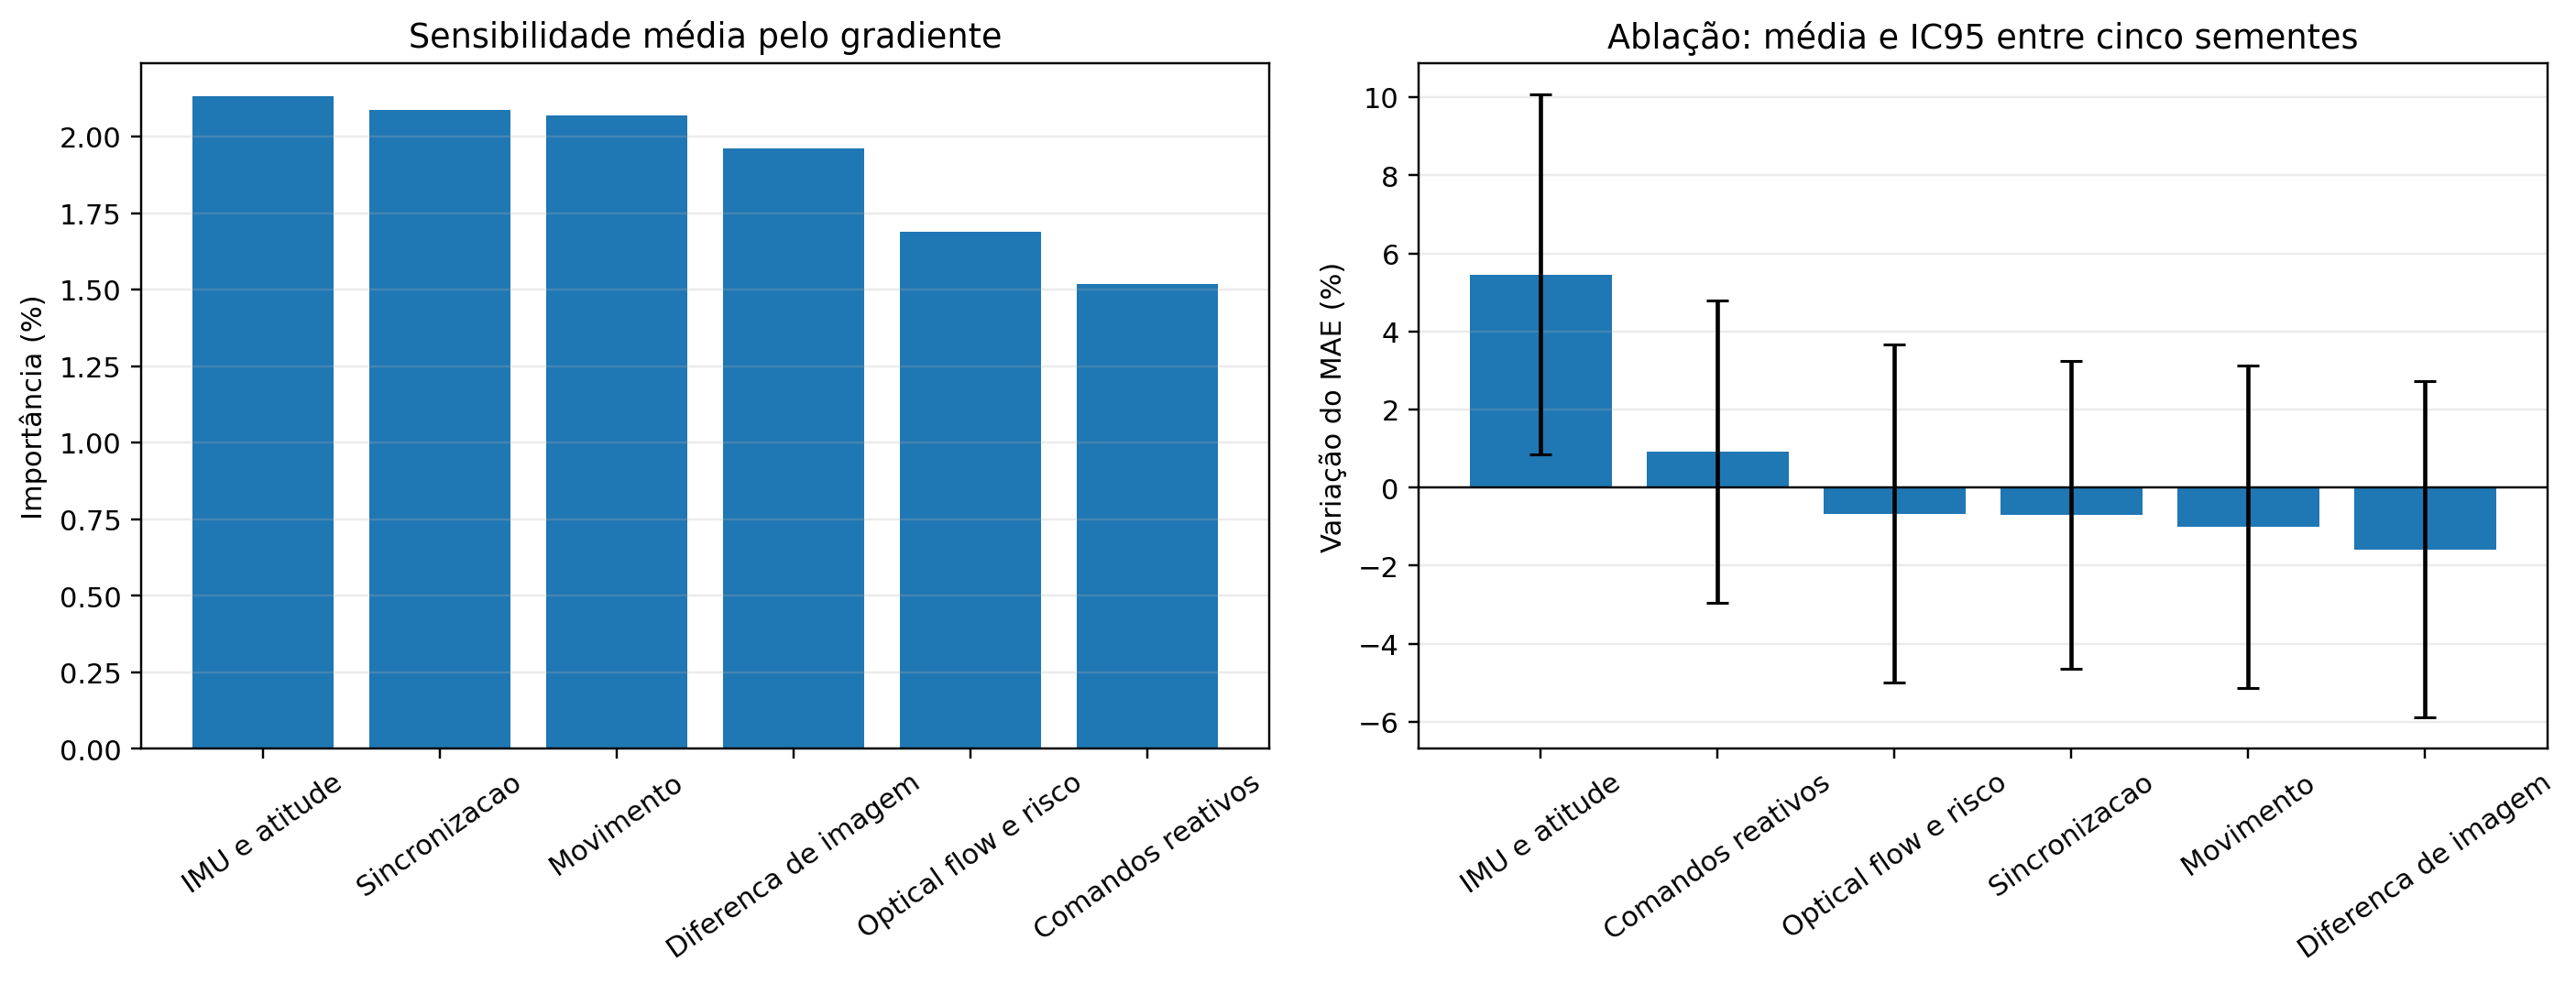
\includegraphics[width=\textwidth]{figuras/resultados_explicabilidade_ablacao.png}
    \caption{Sensibilidade por gradientes e efeito da retirada dos grupos de entradas. Cada configuração usa cinco sementes; as barras resumem os IC95 por alvo, calculados com distribuição $t$ e $n=5$.}
    \label{fig:mono-ablacao}
    \legend{Fonte: elaborado pelo autor.}
\end{figure}

\begin{table}[htb]
\centering
\caption{Variação média do MAE após a retirada de cada grupo.}
\label{tab:mono-ablacao}
\begin{tabular}{lr}
\hline
\textbf{Grupo retirado} & \textbf{$\Delta$ MAE médio (\%)} \\
\hline
IMU e atitude & 5,45 \\
Comandos reativos & 0,92 \\
Fluxo óptico e risco & -0,67 \\
Sincronização & -0,70 \\
Movimento & -1,00 \\
Diferença de imagem & -1,58 \\
\hline
\end{tabular}
\legend{Fonte: elaborado pelo autor a partir de cinco sementes por ablação.}
\end{table}

\subsection{Bateria espacial com profundidade do Gazebo}

As dez execuções completaram os três objetivos, totalizando 30 objetivos alcançados. Houve 156 tentativas de planejamento, 147 sucessos e 132 caminhos adotados. As nove tentativas sem solução não encerraram as missões: o controlador interrompeu o avanço quando necessário e voltou a planejar após novas observações. A bateria registrou 50 vetos de caminho ativo e 50 frenagens concluídas. Nenhum caminho adotado foi classificado como inseguro pelo guardião de referência. Esses números valem para a rota fixa e o cenário simulado avaliados, não demonstram segurança geral. A duração média foi 77,37~s, com desvio de 4,49~s. O intervalo de confiança de 95\% para essa média, calculado com distribuição $t$ e dez execuções, foi de 74,16 a 80,58~s. O planejamento levou em média 99,18~ms, com desvio padrão de 67,14~ms, mediana de 100,72~ms, percentil 95 de 217,30~ms e intervalo observado de 3,69 a 298,91~ms nas 156 tentativas.

Os intervalos das demais métricas usam bootstrap das dez execuções completas, com 10.000 reamostragens e semente 42. Essa unidade evita supor independência entre tentativas da mesma missão. Os IC95 foram: sucesso de planejamento de 90,67\% a 97,40\%; falso espaço livre de 0,289 a 0,342; precisão de ocupação de 1,000 a 1,000; revocação de 0,564 a 0,604; e médias de vetos e frenagens de 3,4 a 6,6 por execução. Eles descrevem somente a variabilidade da rota observada.

\begin{table}[htb]
\centering
\caption{Resultados individuais da bateria espacial de referência.}
\label{tab:mono-bateria-individual}
\resizebox{\textwidth}{!}{%
\begin{tabular}{rrrrrrrr}
\hline
Execução & Duração (s) & Planos (sucesso/tentativa) & Adotados & Vetos & Frenagens & Objetivos & Inseguros \\
\hline
1 & 76,87 & 15/16 & 14 & 6 & 6 & 3 & 0 \\
2 & 73,56 & 14/15 & 13 & 5 & 5 & 3 & 0 \\
3 & 85,97 & 14/17 & 14 & 7 & 7 & 3 & 0 \\
4 & 72,93 & 9/9   & 8  & 1 & 1 & 3 & 0 \\
5 & 84,61 & 22/23 & 19 & 8 & 8 & 3 & 0 \\
6 & 77,79 & 14/14 & 11 & 3 & 3 & 3 & 0 \\
7 & 75,11 & 16/17 & 14 & 4 & 4 & 3 & 0 \\
8 & 73,64 & 15/15 & 15 & 9 & 9 & 3 & 0 \\
9 & 76,52 & 13/13 & 11 & 1 & 1 & 3 & 0 \\
10 & 76,71 & 15/17 & 13 & 6 & 6 & 3 & 0 \\
\hline
Total & 773,71 & 147/156 & 132 & 50 & 50 & 30 & 0 \\
\hline
\end{tabular}}
\legend{Fonte: \path{logs/spatial_final_analysis/final_20260901/reference_runs.csv}.}
\end{table}

\begin{table}[htb]
\centering
\caption{Resumo da bateria espacial final com profundidade do Gazebo.}
\label{tab:mono-bateria}
\begin{tabular}{lr}
\hline
Runs completas & 10/10 \\
Objetivos globais alcançados & 30 \\
Planos bem-sucedidos & 147/156 (94,23\%) \\
Caminhos adotados & 132 \\
Caminhos adotados inseguros & 0 \\
Vetos de caminho ativo & 50 \\
Frenagens concluídas & 50 \\
Duração média & 77,37 $\pm$ 4,49~s \\
Tempo médio de planejamento & 99,18~ms \\
Desvio padrão do planejamento & 67,14~ms \\
Mediana / percentil 95 do planejamento & 100,72 / 217,30~ms \\
\hline
\end{tabular}
\legend{Fonte: relatório final consolidado da auditoria espacial.}
\end{table}

A precisão média de ocupação foi 1,0, a revocação 0,584 e a taxa de falso espaço livre 0,316. Sejam $O_r$ os voxels ocupados do mapa de referência e $F_e$ os voxels classificados como livres no mapa avaliado. A implementação calcula
\[
\mathrm{TFL}=\frac{|O_r\cap F_e|}{|O_r|}.
\]
O denominador contém todos os voxels ocupados da referência, inclusive os que podem estar fora da cobertura do estado parcial avaliado. Assim, 0,316 não significa que o sensor do Gazebo errou em 31,6\%; representa divergência entre mapas com cobertura temporal diferente.

No replay, uma colisão ocorre quando os voxels enumerados conservadoramente ao longo de um caminho executável interceptam $O_r$ depois da inflação de segurança. O teste é discreto e não calcula a distância euclidiana contínua entre a malha do VANT e a geometria do obstáculo. A resolução de 0,75~m e a inflação tornam o critério conservador, mas a evidência permanece restrita à grade. Por isso, a bateria usa a verificação dos caminhos adotados, e não a interpretação isolada da taxa de falso espaço livre.

A Figura~\ref{fig:mono-mapa-astar} apresenta uma projeção no plano NED da primeira execução da bateria. Os pontos ocupados foram filtrados pela faixa de voo; as linhas mostram os caminhos efetivamente adotados.

\begin{figure}[htb]
    \centering
    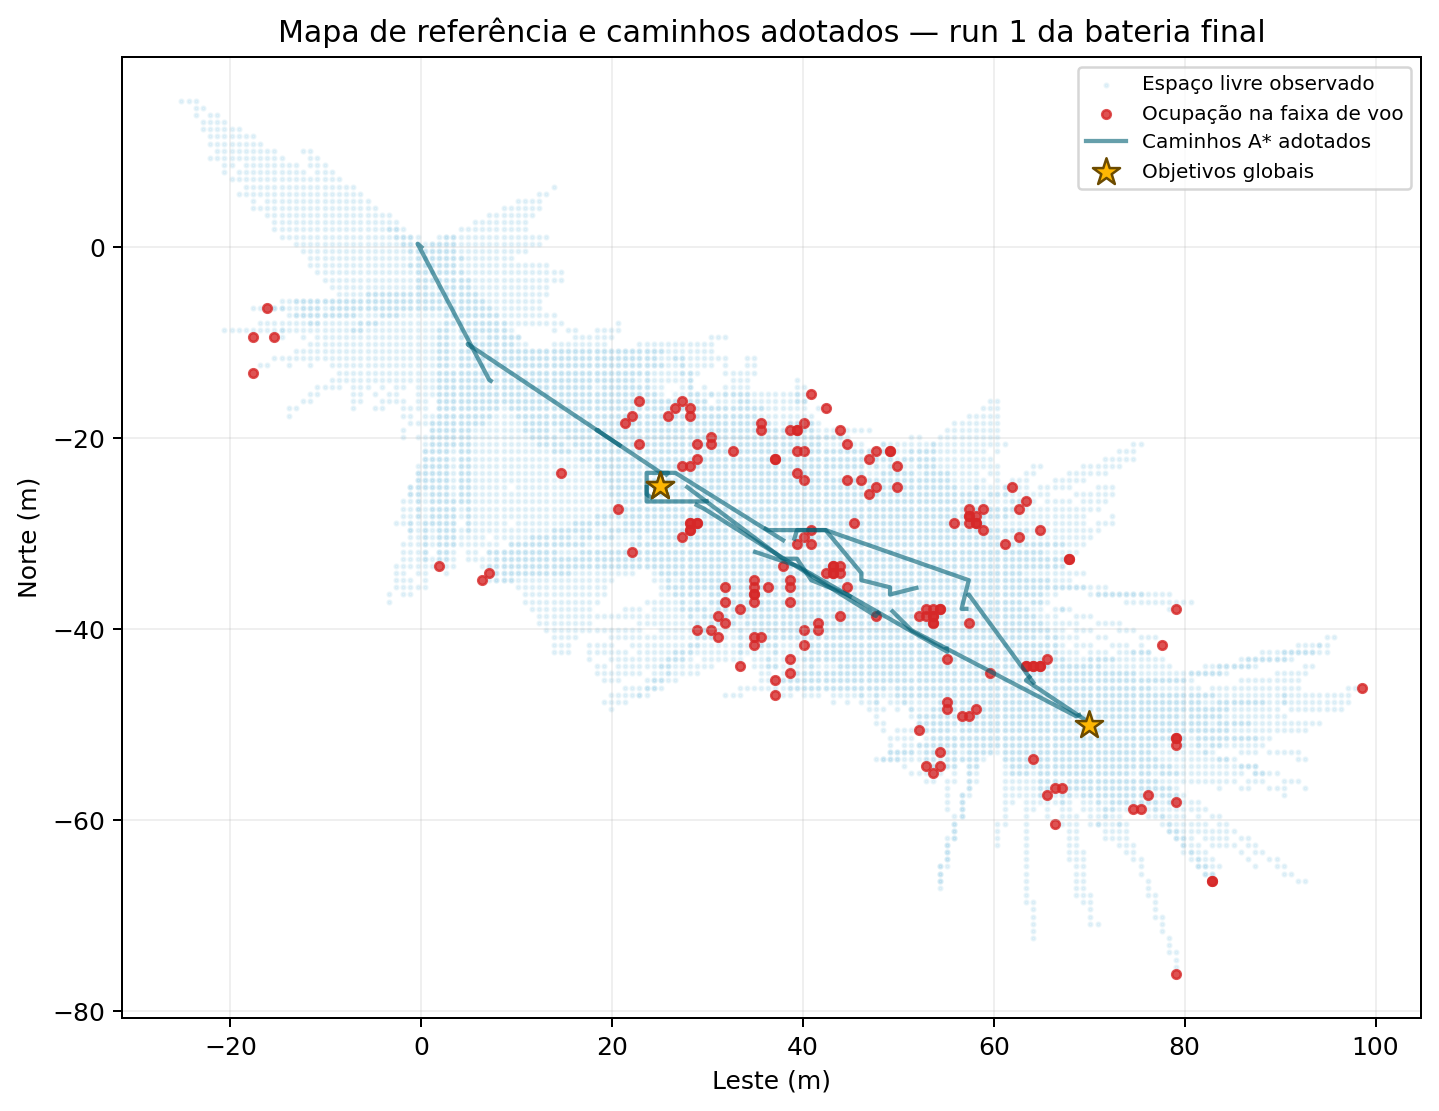
\includegraphics[width=\textwidth]{figuras/resultados_mapa_astar.png}
    \caption{Mapa de referência e caminhos A* adotados na primeira execução da bateria final.}
    \label{fig:mono-mapa-astar}
    \legend{Fonte: elaborado pelo autor a partir dos registros da bateria.}
\end{figure}

\subsection{Portão monocular}

A Tabela~\ref{tab:mono-versoes} resume as versões v12--v19. O sucesso de planejamento, a taxa de falso espaço livre e as colisões correspondem ao conjunto espacial primário usado em cada versão e, portanto, servem para decisão de portão, não para uma comparação em um teste único idêntico. As versões v12 e v13 usaram o conjunto histórico disponível naquela fase. A partir da v14, adotou-se a terceira execução da bateria final de referência, criada posteriormente e mantida como conjunto primário até a v19. Essa mudança acompanha a evolução cronológica do protocolo; os números entre v13 e v14 não formam uma comparação controlada entre arquiteturas.

\begin{table}[htb]
\centering
\caption{Profundidade e resultado espacial das versões monoculares.}
\label{tab:mono-versoes}
\resizebox{\textwidth}{!}{%
\begin{tabular}{lrrrrl}
\hline
\textbf{Versão} & \textbf{MAE (m)} & \textbf{AbsRel} & \textbf{Sucesso planos} & \textbf{Falso livre} & \textbf{Colisões} \\
\hline
v12 & 1,283 & 0,151 & 27,8\% & 0,367 & 0 \\
v13 & 1,242 & 0,156 & 38,9\% & 0,390 & 2 \\
v14 & 1,270 & 0,156 & 47,1\% & 0,431 & 1 \\
v15 & 1,726 & 0,199 & 41,2\% & 0,304 & 0 \\
v16 & 1,383 & 0,152 & 52,9\% & 0,291 & 1 \\
v17 & 1,498 & 0,159 & 35,3\% & 0,184 & 0 \\
v18 & 1,292 & 0,141 & 52,9\% & 0,263 & 1 \\
v19 & 1,286 & 0,141 & 41,2\% & 0,184 & 0 \\
\hline
\end{tabular}}
\legend{Fonte: relatório final consolidado da auditoria espacial.}
\end{table}

Sete versões passaram pelo critério por pixel; a v15 foi reprovada apenas no MAE da faixa de 5 a 10~m: 1,648~m diante do limite de 1,5~m. Nenhuma aprovou o portão espacial completo. O estimador monocular final avaliado, v19, integrou 77 quadros, abaixo do mínimo de 100, obteve 41,2\% de sucesso de planejamento, abaixo de 80\%, e falso espaço livre de 0,184, acima de 0,10. A execução era completa e recebeu 1.227 quadros de câmera, mas o processamento ocorria a cada dez quadros; entre os quadros candidatos, 45 não tinham profundidade sincronizada e nenhum foi rejeitado por idade. Assim, 77 quadros foram efetivamente integrados e persistidos.

Nos quatro conjuntos secundários, os pares quadros, sucesso de planejamento e falso espaço livre foram, respectivamente: 80, 42,9\% e 0,206 na sexta execução da bateria; 68, 88,2\% e 0,305 na décima; 122, 36,4\% e 0,182 na execução antiga independente; e 117, 16,7\% e 0,275 na execução histórica reservada. Nenhum aprovou o portão completo. As duas execuções antigas atingiram o mínimo de quadros, mas reprovaram os limites de sucesso e falso espaço livre. O resultado confirma a insuficiência espacial fora do conjunto primário.

A decisão primária não é sensível a pequenas variações dos limiares. Para que os valores observados da v19 fossem aprovados sem alterar o modelo, seria necessário reduzir ao mesmo tempo o mínimo de quadros de 100 para 77, o sucesso mínimo de 80\% para 41,2\% e elevar o falso espaço livre máximo de 10\% para 18,4\%. Logo, a reprovação permanece para perturbações locais dos limites congelados.

O artefato avaliado foi \path{models/depth_anything_v2_metric_baylands_vits_v19_final_686x518_fp32.onnx}, com SHA-256 \texttt{b56cbb291b8fade37a0b5f298fdd4bbe5e45de05f92628a1956828b0fc902dc4}. A configuração de melhor posição no portão foi \texttt{v19\_scale1p0\_shift1p2}: escala 1,0, deslocamento conservador de 1,2~m, margem livre de 3,0~m, incerteza ocupada de 1,5~m e banda e inflação verticais de 0,10~m. Na avaliação offline de 24 quadros, a inferência da v19 levou 286,7~ms em média e 292,0~ms no percentil 95. Esse valor satisfaz o limite experimental de 400~ms, mas não demonstra operação em tempo real em outras plataformas. O planejamento foi medido na bateria de referência e a inferência no ensaio monocular offline. Como os valores vêm de execuções diferentes, eles não podem ser somados para estimar a latência total. O intervalo entre receber a imagem, atualizar o mapa, planejar e publicar o caminho não foi instrumentado nesta bateria.

As Figuras~\ref{fig:mono-comparacao-profundidade}, \ref{fig:mono-comparacao-profundidade-floresta} e \ref{fig:mono-falso-livre} mostram o efeito da estimativa. A primeira usa o quadro 73, que apresentou o maior MAE entre os 77 quadros persistidos; trata-se de um caso crítico ilustrativo, não do comportamento médio. A segunda acrescenta o quadro 69 de outra execução, capturado com a câmera nivelada sob copas densas e diante de vários troncos. A terceira projeta no plano NED os 84 voxels que a referência marcou como ocupados e a v19 integrou como livres, correspondentes a 18,38\% dos 457 voxels ocupados de referência. Na projeção 2D, voxels de alturas diferentes podem se sobrepor. As divergências não significam 84 colisões.

\begin{figure}[htb]
    \centering
    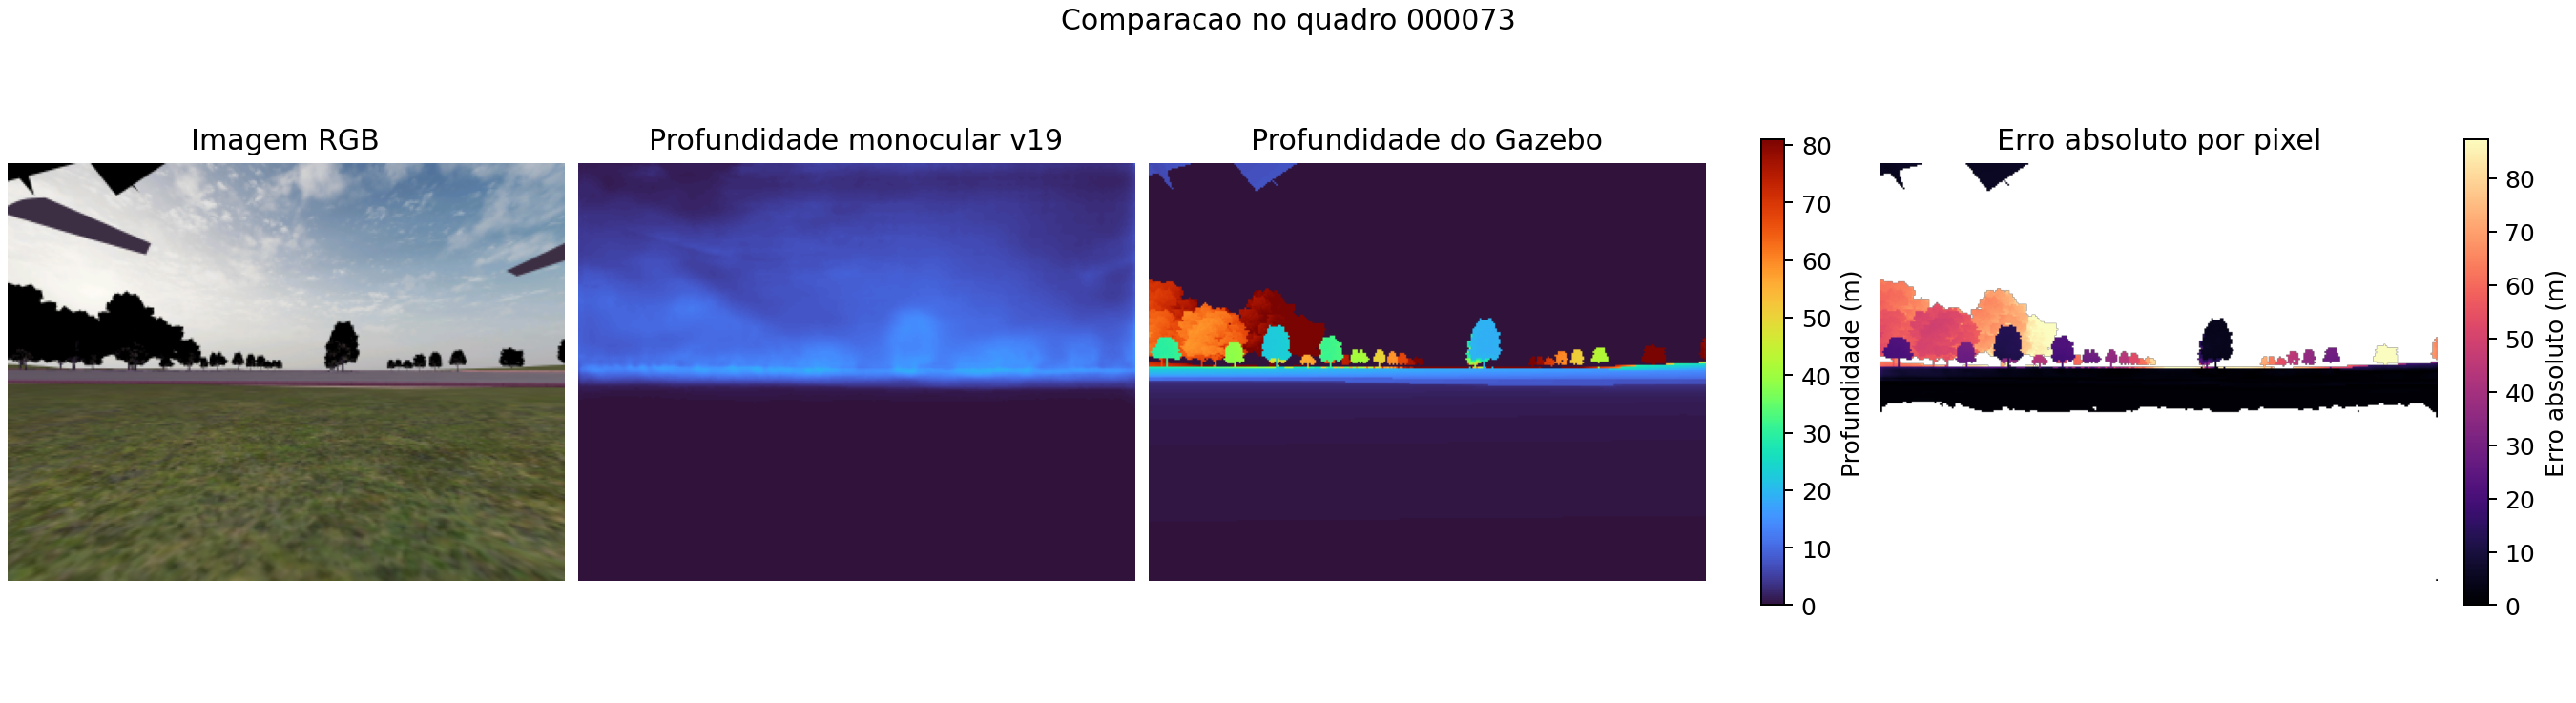
\includegraphics[width=\textwidth]{figuras/resultados_comparacao_profundidade_v19.png}
    \caption{Comparação entre RGB, profundidade monocular v19, profundidade do Gazebo e erro absoluto por pixel.}
    \label{fig:mono-comparacao-profundidade}
    \legend{Fonte: elaborado pelo autor a partir do replay offline do quadro 73.}
\end{figure}

\begin{figure}[htb]
    \centering
    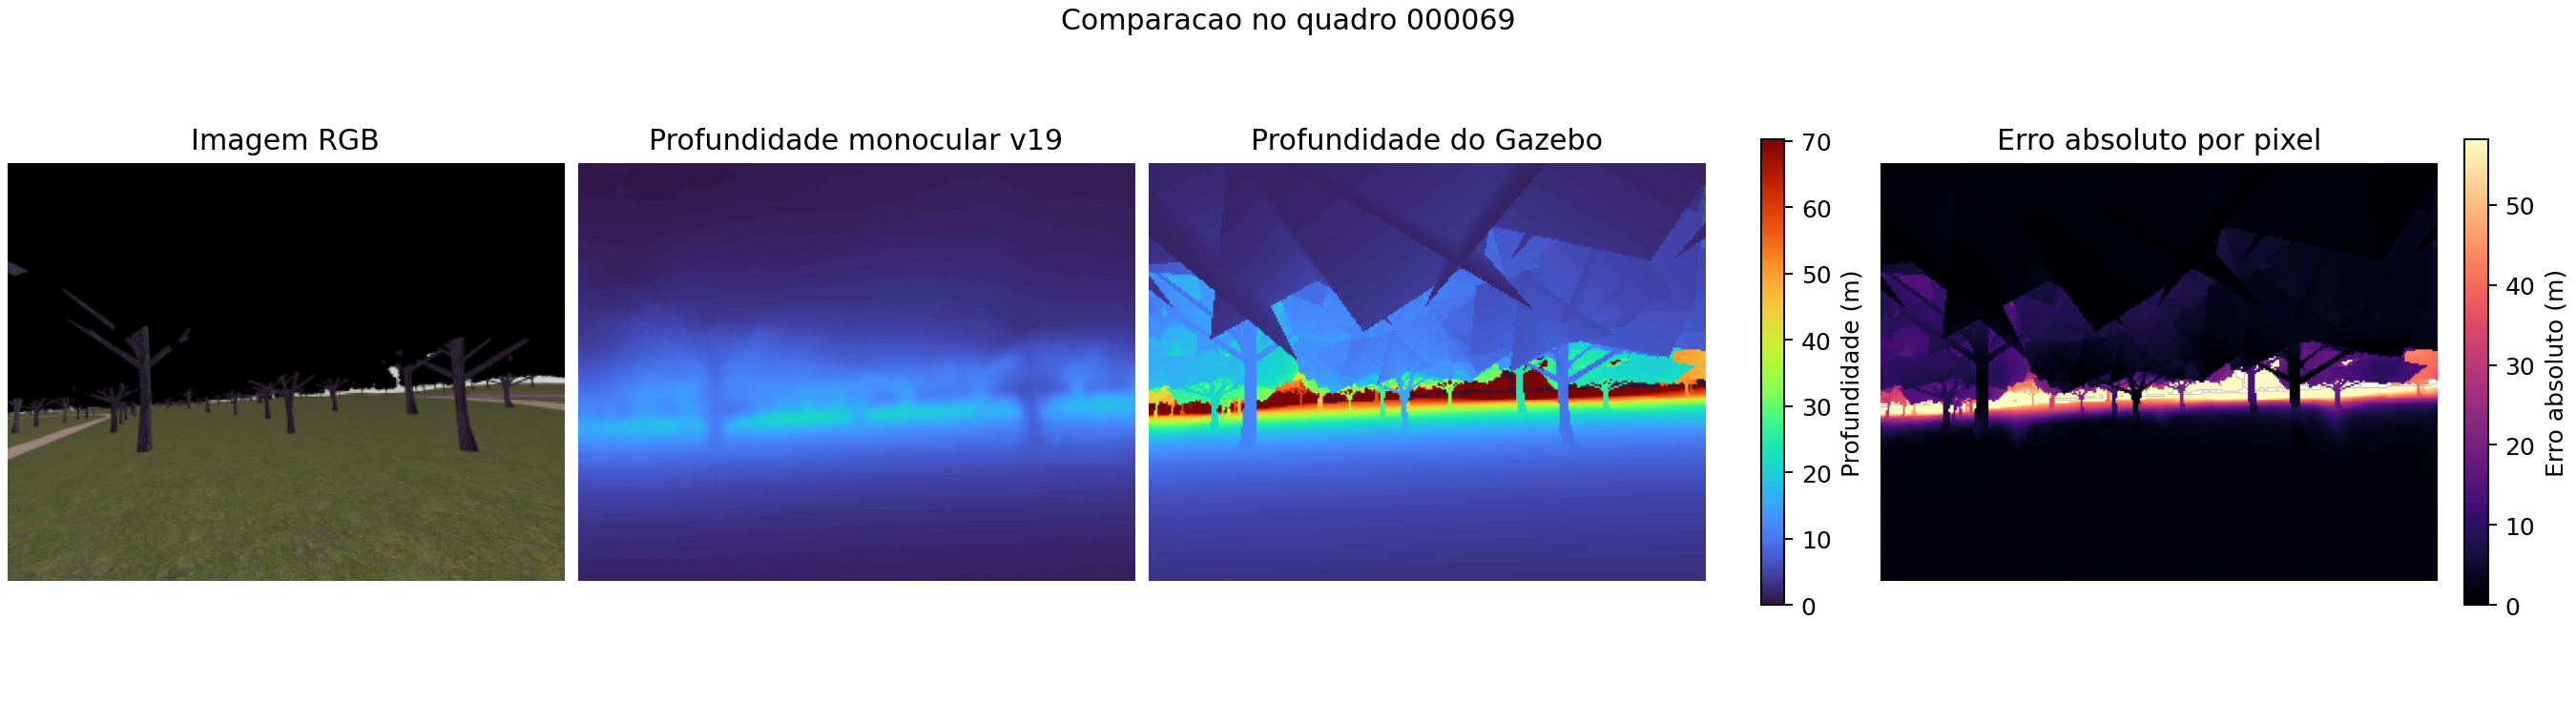
\includegraphics[width=\textwidth]{figuras/resultados_comparacao_profundidade_v19_floresta.png}
    \caption{Comparação entre RGB, profundidade monocular v19, profundidade do Gazebo e erro absoluto por pixel em um quadro capturado dentro da área arborizada.}
    \label{fig:mono-comparacao-profundidade-floresta}
    \legend{Fonte: elaborado pelo autor a partir do replay offline do quadro 69 da execução \texttt{run\_20260819\_185210\_952450}.}
\end{figure}

\begin{figure}[htb]
    \centering
    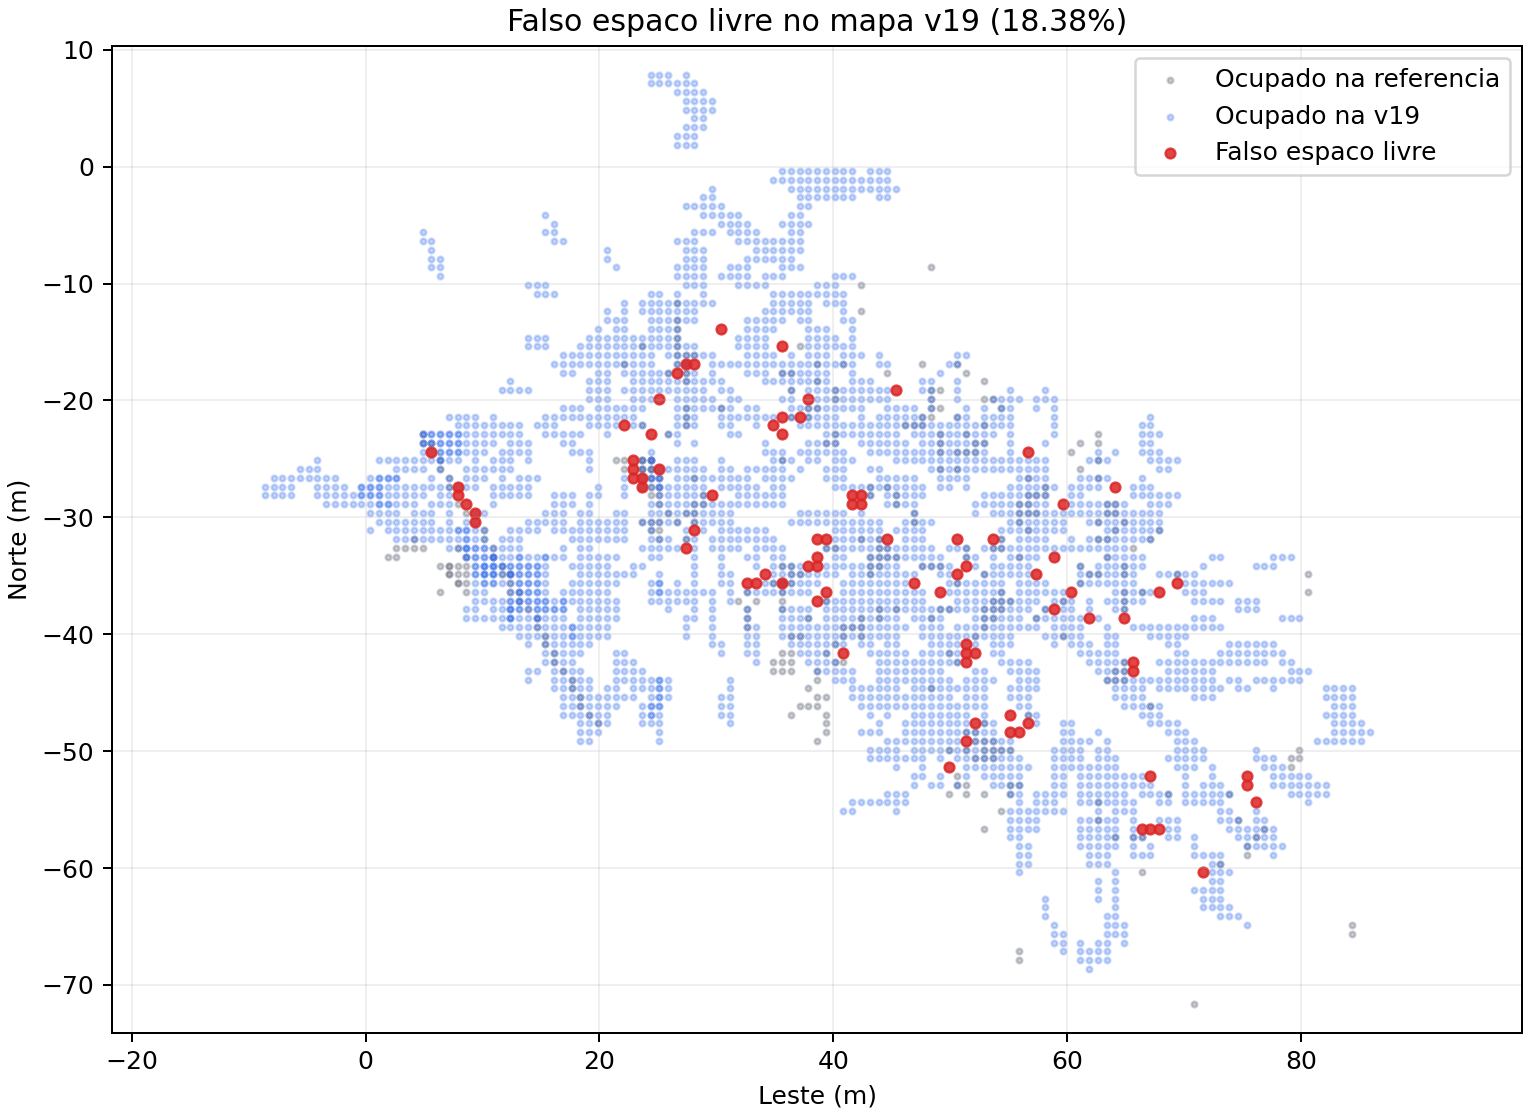
\includegraphics[width=0.82\textwidth]{figuras/resultados_falso_espaco_livre_v19.png}
    \caption{Projeção no plano NED dos falsos espaços livres produzidos pela v19.}
    \label{fig:mono-falso-livre}
    \legend{Fonte: elaborado pelo autor a partir dos 77 quadros do conjunto primário.}
\end{figure}

\section{Considerações finais}

O eixo tabular mostrou ganhos modestos, estabilidade entre sementes e limites claros da representação resumida. O eixo espacial mostrou que a geometria e o planejamento funcionam com profundidade do Gazebo na rota e no cenário simulados, mas que a profundidade monocular disponível ainda não sustenta o mesmo nível de segurança. Os obstáculos do experimento eram estáticos; objetos em movimento não foram avaliados. A reprovação do portão preserva esse resultado sem transformar um diagnóstico offline em autorização de voo.
